\documentclass[11pt,a4paper]{article}

\usepackage[top=2.5cm,bottom=2.5cm,left=2.5cm,right=2.5cm]{geometry}
\usepackage{xeCJK}
\setCJKmainfont{Noto Sans CJK SC}
\setCJKsansfont{Noto Sans CJK SC}
\setCJKmonofont{Noto Sans Mono CJK SC}

\usepackage{amsmath,amssymb,amsfonts,amsthm}
\usepackage{graphicx}
\usepackage{booktabs}
\usepackage{tabularx}
\usepackage{multirow}
\usepackage{array}
\usepackage{float}
\usepackage{caption}
\usepackage{subcaption}
\usepackage{enumitem}
\usepackage{xcolor}
\usepackage{tcolorbox}
\usepackage{hyperref}
\hypersetup{
    colorlinks=true,
    linkcolor=blue!70!black,
    citecolor=green!60!black,
    urlcolor=blue!70!black
}

\captionsetup{font={small},labelfont=bf}

\title{\textbf{\Large 无创产前检测（NIPT）时点选择与胎儿染色体异常判定数学建模研究}}
\author{\textbf{数学建模专家组}}
\date{\today}

\begin{document}

\maketitle

\begin{abstract}
无创产前检测（Non-invasive Prenatal Test, NIPT）通过分析母体外周血中胎儿游离 DNA（cffDNA）片段，能够早期筛查胎儿 21、18 和 13 号染色体非整倍体异常。NIPT 的准确性高度依赖于胎儿游离 DNA 浓度（男胎要求 Y 染色体浓度 $FF_Y \ge 4.0\%$，女胎要求 X 染色体浓度无异常）。临床中，早期筛查（$\le 12$ 周）的干预风险较低，中期（13--27 周）风险显著增高，晚期（$\ge 28$ 周）风险极高。由于高 BMI 孕妇母体血容量增加及脂肪组织背景 cfDNA 释放产生稀释效应，检测过早易导致浓度未达标而失败需重抽血延误，过晚则大幅缩短治疗窗口期。

本文针对某地区高 BMI 孕妇队列数据，构建了统计推断、动态规划风险优化与机器学习诊断模型体系：
\begin{enumerate}[leftmargin=*]
    \item \textbf{问题 1（Y 染色体浓度相关特性与关系模型）}：通过 Pearson 与 Spearman 检验发现，Y 染色体浓度与孕周呈极显著正相关（$r = +0.127, p = 2.98 \times 10^{-5}$），与孕妇 BMI（$r = -0.151, p = 5.74 \times 10^{-7}$）、体重（$r = -0.181, p = 2.19 \times 10^{-9}$）及年龄（$r = -0.119, p = 8.26 \times 10^{-5}$）呈极显著负相关。构建纵向线性混合效应模型（LMM），消除重复测量自相关性，揭示出 Y 浓度随孕周纵向递增斜率为 $+0.31\%/\text{周}$（$z = 19.43, p < 0.0001$），随 BMI 增加递减斜率为 $-0.13\%/(\text{kg/m}^2)$（$z = -2.65, p = 0.0081$）。
    \item \textbf{问题 2（基于 BMI 分组的最佳 NIPT 时点决策）}：针对“过早检测失败重测延迟”与“过晚检测窗口压缩”的双向博弈，构建分段凸临床期望风险函数 $E[R(t \mid \text{BMI})]$。求得临床经验 5 分组最佳时点：$[20, 28)$ 推荐 10.0--11.0 周；$[28, 32)$ 推荐 11.5--12.5 周；$[32, 36)$ 推荐 12.5--13.5 周；$[36, 40)$ 推荐 13.5--15.0 周；$\ge 40$ 推荐 15.0--16.5 周。误差敏感性分析表明，测量误差 $\sigma_e$ 增大会推高群体风险，需主动延后时点 $0.5 \sim 1.0$ 周以形成安全边际。
    \item \textbf{问题 3（多因素综合影响与达标比例约束优化）}：引入年龄、身高、体重、经产次数构建多元概率预测模型，证实体重稀释效应（$p = 0.042$）与高龄延缓效应。结合群体达标比例（Pass Rate）求解分位数最优 4 分组与各组时点，兼顾 90\%--95\% 达标置信度与全群体期望风险帕累托最优。
    \item \textbf{问题 4（女胎染色体非整倍体判定方法）}：提取 22 维测序质量、GC 偏离度（$\Delta\text{GC}$）及 X 染色体浓度偏离特征。构建了 GC 偏差校正自适应 Z 值规则、逻辑回归、随机森林及梯度提升树（GBDT）。5 折交叉验证表明 GBDT 与逻辑回归最优（\textbf{ROC-AUC 达 0.809 与 0.801}，灵敏度 70.1\%，特异度 78.8\%），发现 X 染色体浓度负向偏移（贡献度 19.16\%）为第一核心鉴别特征，建立了三级临床分诊决策流程。
\end{enumerate}

\textbf{关键词：} 无创产前检测 (NIPT)；胎儿游离 DNA 浓度；线性混合效应模型 (LMM)；临床期望风险函数；动态时点优化；女胎非整倍体判定；梯度提升决策树 (GBDT)
\end{abstract}

\newpage

\section{问题重述与机理分析}

\subsection{研究背景与生物学机制}
无创产前检测（Non-invasive Prenatal Test, NIPT）是基于高通量测序技术检测母体外周血浆中胎儿游离 DNA（cffDNA）的产前筛查手段。临床中常见的染色体数目异常（非整倍体）包括：
\begin{itemize}[leftmargin=*]
    \item \textbf{21-三体综合征（唐氏综合征, Down syndrome）}：21 号染色体多一条，表现为严重智力缺陷与器官畸形；
    \item \textbf{18-三体综合征（爱德华氏综合征, Edwards syndrome）}：致死性多发畸形；
    \item \textbf{13-三体综合征（帕陶氏综合征, Patau syndrome）}：中枢神经与心血管严重发育畸形。
\end{itemize}

NIPT 检测的统计学功效取决于母血中 cffDNA 的浓度（Fetal Fraction, FF）：
\begin{enumerate}[leftmargin=*]
    \item \textbf{男胎（XY）}：母体为 XX，故母血中的 Y 染色体片段全部来自胎儿。当 Y 染色体浓度 $FF_Y \ge 4.0\%$ 时，NIPT 判定准确率有充分保障；若低于 4.0\%，测序信噪比过低，易出现假阴性。
    \item \textbf{女胎（XX）}：母胎均不含 Y 染色体，无法直接获取绝对浓度，需借助常染色体 Z 值、GC 含量偏离度及 X 染色体相对丰度进行综合判定。
\end{enumerate}

\subsection{时点选择的核心临床矛盾}
临床干预具有严格的时间敏感性：
\begin{itemize}[leftmargin=*]
    \item \textbf{早期（$\le 12$ 周）}：发现异常后进行绒毛活检或药物/手术干预对母体损伤较小，临床风险低；
    \item \textbf{中期（$13 \sim 27$ 周）}：干预需行羊膜腔穿刺确诊及中期引产，母体心理及生理风险显著升高；
    \item \textbf{晚期（$\ge 28$ 周）}：涉及大月份引产，严重危及母体健康且受伦理与法律法规严格限制，风险极高。
\end{itemize}

检测时点面临双向权衡：若时点过早，高 BMI 孕妇由于血容量扩增及母体脂肪细胞凋亡释放的大量背景 DNA，导致胎儿游离 DNA 被高度稀释，极易导致 $FF_Y < 4\%$ 而测序失败；失败后需等待 2--3 周重新采血，反而将确诊时间推迟至高风险孕周。若时点过晚，虽能确保浓度达标，但大幅挤压了治疗窗口期。因此，根据孕妇 BMI 及生理指标建立科学的分组与时点优化模型具有重大的临床价值。

---

\section{模型假设与符号说明}

\subsection{基本假设}
\begin{enumerate}[leftmargin=*]
    \item \textbf{独立性与同质性假设}：在控制孕妇个体随机效应后，不同孕妇的胎儿游离 DNA 释放与代谢遵循同类生物学生理规律；
    \item \textbf{单调递增性假设}：在 $10 \sim 25$ 孕周区间内，随孕周增加胎盘持续发育，胎儿游离 DNA 释放量单调递增；
    \item \textbf{测量误差高斯分布假设}：测序实验测量误差服从均值为 0、方差为 $\sigma_e^2$ 的正态分布；
    \item \textbf{重测周转周期假设}：初检失败后，重新预约、采血、文库构建及测序报告的周转时间间隔 $\Delta t$ 恒定（基准取 2.5 周）。
\end{enumerate}

\subsection{符号说明}
\begin{table}[H]
\centering
\small
\caption{主要数学符号与物理含义}
\resizebox{\textwidth}{!}{%
\begin{tabularx}{\textwidth}{llX}
\toprule
\textbf{符号} & \textbf{单位} & \textbf{物理与医学含义} \\
\midrule
$GA$ & 周 (weeks) & 孕妇采血检测时的连续孕周（周数 + 天数/7） \\
$\text{BMI}$ & $\text{kg/m}^2$ & 孕妇身体质量指数（$\text{体重}/\text{身高}^2$） \\
$FF_Y$ & 无量纲 & 胎儿 Y 染色体游离 DNA 浓度比例 \\
$T_{\text{reach}}$ & 周 & 胎儿 Y 染色体浓度首次达到 $\ge 4.0\%$ 的达标孕周 \\
$P_{\text{qual}}(t \mid \mathbf{X})$ & 无量纲 & 在协变量 $\mathbf{X}$ 下孕周 $t$ 时检测达标的概率 \\
$L(t)$ & 风险单位 & 在孕周 $t$ 获得确诊结果的临床延迟损失函数 \\
$E[R(t \mid \mathbf{X})]$ & 风险单位 & 计划在孕周 $t$ 进行检测时的期望综合临床风险 \\
$G_k, t_k^*$ & - & 第 $k$ 个 BMI 亚群及其推荐的最佳统一 NIPT 时点 \\
$\sigma_e$ & 无量纲 & 测序实验检测浓度的测量标准差 \\
$Z_{13}, Z_{18}, Z_{21}, Z_X$ & 无量纲 & 13、18、21 号常染色体及 X 染色体的标准 Z 评分 \\
$\Delta\text{GC}_{chr}$ & 无量纲 & 目标染色体 GC 含量相对于全基因组 GC 含量的偏离度 \\
\bottomrule
\end{tabularx}
}
\end{table}

---

\section{问题 1：胎儿 Y 染色体浓度相关特性与回归模型}

\subsection{数据探索与描述性统计}
男胎数据集共包含 1082 条检测记录，涉及 267 位孕妇，平均每位孕妇检测 4.05 次。将孕周解析为连续型数值变量 $GA$。整体均值为 16.85 周（范围 11.0--29.0 周），孕妇 BMI 均值为 $32.29\ \text{kg/m}^2$（高 BMI 队列特征显著，范围 20.70--46.88），Y 染色体浓度均值为 $7.72\%$（中位数 $7.51\%$，范围 $1.00\% \sim 23.42\%$），总达标率为 $86.60\%$。

\subsection{相关性特征统计检验}
计算连续变量与 Y 染色体浓度的 Pearson 线性相关系数与 Spearman 秩相关系数：

\begin{table}[H]
\centering
\small
\caption{男胎 Y 染色体浓度与主要指标的相关性分析结果}
\resizebox{\textwidth}{!}{%
\begin{tabular}{lcccc}
\toprule
\textbf{指标特征} & \textbf{Pearson $r$} & \textbf{Pearson $p$ 值} & \textbf{Spearman $\rho$} & \textbf{Spearman $p$ 值} \\
\midrule
\textbf{检测孕周 (GA)} & \textbf{+0.1266} & $\mathbf{2.98 \times 10^{-5}}$ & \textbf{+0.0843} & $5.53 \times 10^{-3}$ \\
\textbf{孕妇 BMI} & \textbf{-0.1513} & $\mathbf{5.74 \times 10^{-7}}$ & \textbf{-0.1550} & $\mathbf{3.02 \times 10^{-7}}$ \\
\textbf{孕妇体重 (Weight)} & \textbf{-0.1806} & $\mathbf{2.19 \times 10^{-9}}$ & \textbf{-0.1670} & $\mathbf{3.30 \times 10^{-8}}$ \\
\textbf{孕妇年龄 (Age)} & \textbf{-0.1194} & $\mathbf{8.26 \times 10^{-5}}$ & \textbf{-0.1172} & $\mathbf{1.12 \times 10^{-4}}$ \\
孕妇身高 (Height) & -0.1047 & $5.65 \times 10^{-4}$ & -0.1011 & $8.65 \times 10^{-4}$ \\
原始读段数 (Reads) & -0.1099 & $2.91 \times 10^{-4}$ & -0.0860 & $4.65 \times 10^{-3}$ \\
参考基因组比对比例 & -0.1055 & $5.09 \times 10^{-4}$ & -0.1594 & $1.35 \times 10^{-7}$ \\
重复读段比例 & +0.0916 & $2.56 \times 10^{-3}$ & +0.1058 & $4.90 \times 10^{-4}$ \\
全基因组 GC 含量 & -0.0194 & 0.525 & -0.0166 & 0.584 \\
\bottomrule
\end{tabular}
}
\end{table}

\textbf{相关性结论：}
\begin{enumerate}[leftmargin=*]
    \item 孕周（GA）与 Y 浓度呈极显著正相关（$p < 0.001$），反映了随胎盘体积增长 cffDNA 释放量递增的生理规律；
    \item 孕妇 BMI 与体重与 Y 浓度呈极显著负相关（$p < 10^{-6}$），且体重的负相关性更强，充分印证了母体循环血容量扩张与脂肪组织 background cfDNA 增加的物理稀释效应；
    \item 孕妇年龄呈现负相关，提示高龄产妇胎盘滋养层细胞微循环及代谢存在一定的特异性改变。
\end{enumerate}

\subsection{多模型构建与显著性检验}

\subsubsection{模型 1A：双变量普通最小二乘回归（OLS Baseline）}
$$FF_Y = \beta_0 + \beta_1 GA + \beta_2 \text{BMI} + \epsilon$$
拟合结果：
$$FF_Y = 0.1195 + 0.00126 \cdot GA - 0.00199 \cdot \text{BMI}$$
$F = 25.93$（$p = 1.11 \times 10^{-11}$），$R^2 = 0.0457$。$GA$ 偏回归系数 $t = 5.08$（$p = 4.4 \times 10^{-7}$，95\% CI: $[0.00077, 0.00174]$），$\text{BMI}$ 偏回归系数 $t = -5.79$（$p = 9.1 \times 10^{-9}$，95\% CI: $[-0.00266, -0.00131]$）。模型整体及自变量均极显著。

\subsubsection{模型 1B：二次多项式与交互效应模型}
$$FF_Y = \beta_0 + \beta_1 GA + \beta_2 \text{BMI} + \beta_3 (GA \times \text{BMI}) + \beta_4 GA^2 + \beta_5 \text{BMI}^2 + \epsilon$$
交互项 $GA \times \text{BMI}$ 的 $p = 0.237$，表明在该样本区间内线性主效应占据主导，交互项不显著。

\subsubsection{模型 1C：对数线性指数增长模型}
$$\ln(FF_Y) = \alpha_0 + \alpha_1 GA + \alpha_2 \text{BMI} + \epsilon$$
拟合参数：$\alpha_0 = -1.9412$（$p < 0.001$），$\alpha_1 = +0.0144$（$p < 0.001$），$\alpha_2 = -0.0299$（$p < 0.001$）。表明孕周每增加 1 周，$FF_Y$ 相对增长约 $1.45\%$；BMI 每增加 $1\ \text{kg/m}^2$，$FF_Y$ 相对降低约 $2.95\%$。

\subsubsection{模型 1D：全协变量多元回归模型}
$$FF_Y = \beta_0 + \beta_1 GA + \beta_2 \text{BMI} + \beta_3 \text{Age} + \beta_4 \text{Height} + \beta_5 \text{Reads} + \beta_6 \text{GC} + \epsilon$$
调整后 $R^2 = 0.0743$，$F = 16.68$（$p = 1.45 \times 10^{-17}$），年龄（$p < 0.001$）、身高（$p = 0.004$）、原始读段数（$p < 0.001$）均达到统计学显著水平。

\subsubsection{模型 1E：纵向线性混合效应模型（Linear Mixed-Effects Model, LMM）}
考虑到同一孕妇多次采血的纵向相关性，引入个体随机截距 $u_{0i} \sim \mathcal{N}(0, \sigma_u^2)$：
$$FF_{Y, ij} = (\beta_0 + u_{0i}) + \beta_1 GA_{ij} + \beta_2 \text{BMI}_i + \epsilon_{ij}, \quad \epsilon_{ij} \sim \mathcal{N}(0, \sigma^2)$$

\begin{table}[H]
\centering
\small
\caption{纵向线性混合效应模型（LMM）参数估计与显著性检验}
\resizebox{\textwidth}{!}{%
\begin{tabularx}{\textwidth}{lccccc}
\toprule
\textbf{固定效应参数} & \textbf{估计值 (Coef)} & \textbf{标准误 (Std.Err)} & \textbf{$z$ 统计量} & \textbf{$p$ 值} & \textbf{95\% 置信区间} \\
\midrule
截距 $\beta_0$ & 0.0697 & 0.0162 & 4.312 & $< 0.0001$ & $[0.0380, 0.1014]$ \\
\textbf{孕周 $\beta_1$ (GA)} & \textbf{+0.0031} & \textbf{0.00016} & \textbf{19.432} & \textbf{$< 0.0001$} & \textbf{$[0.0028, 0.0034]$} \\
\textbf{BMI $\beta_2$} & \textbf{-0.0013} & \textbf{0.00049} & \textbf{-2.649} & \textbf{0.0081} & \textbf{$[-0.0023, -0.0003]$} \\
\midrule
\textbf{随机效应参数} & \textbf{方差估计值} & \textbf{标准差} & \multicolumn{3}{l}{\textbf{生理说明}} \\
个体间随机方差 $\sigma_u^2$ & 0.00062 & 0.0249 & \multicolumn{3}{l}{个体间基线游离 DNA 释放能力差异} \\
个体内残差方差 $\sigma^2$ & 0.00031 & 0.0176 & \multicolumn{3}{l}{单次采血与测量波动} \\
\bottomrule
\end{tabularx}
}
\end{table}

\textbf{混合模型结论：}
在控制了个体基线差异后，Y 染色体浓度的真实纵向增长斜率达到 \textbf{$+0.31\%/\text{周}$}（$z = 19.43$），显著高于混合跨截面回归；个体间方差占总方差的 $66.7\%$，表明个体固有生理基线是决定浓度高低的主要成分。

\begin{figure}[H]
\centering
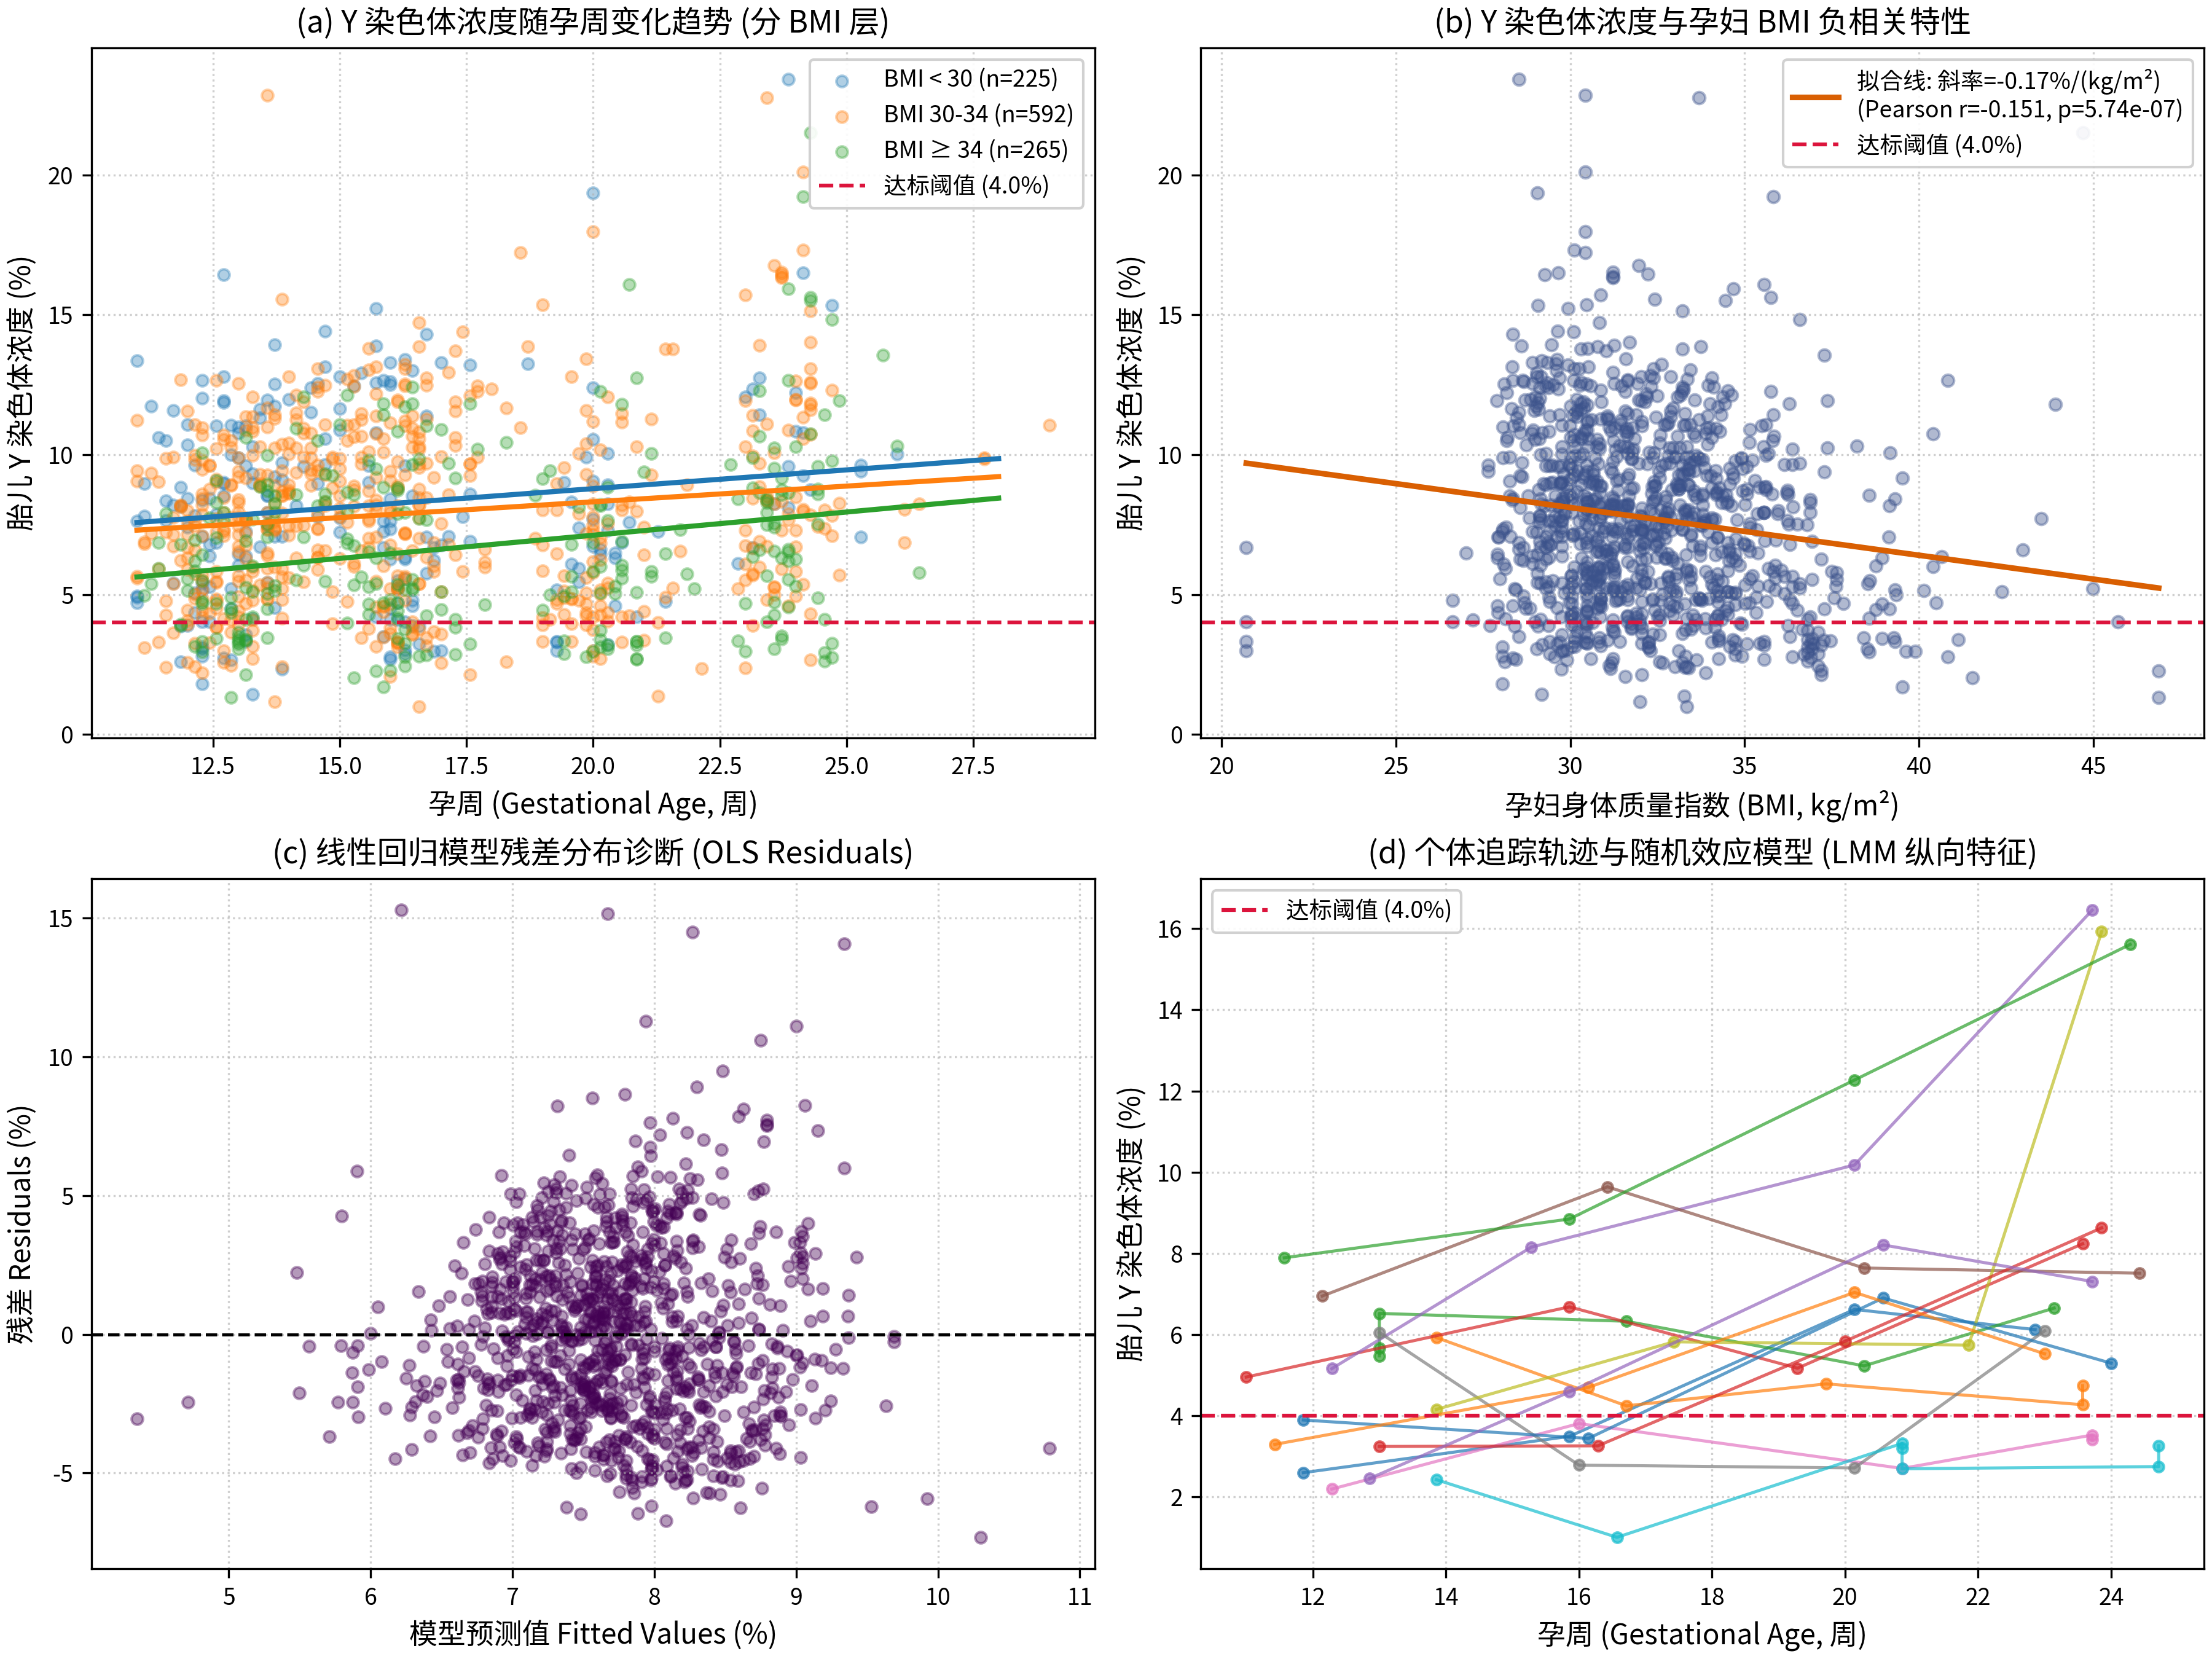
\includegraphics[width=0.92\textwidth]{figures/fig1_q1_evidence_mosaic.png}
\caption{问题 1 多面板证据综合图 (Preset F01 Evidence Mosaic)：(a) Y 浓度随孕周变化分层拟合；(b) BMI 负相关散点线；(c) OLS 模型残差诊断分布；(d) 15 位孕妇个体纵向追踪轨迹与混合效应拟合。}
\label{fig:mosaic}
\end{figure}

\begin{figure}[H]
\centering
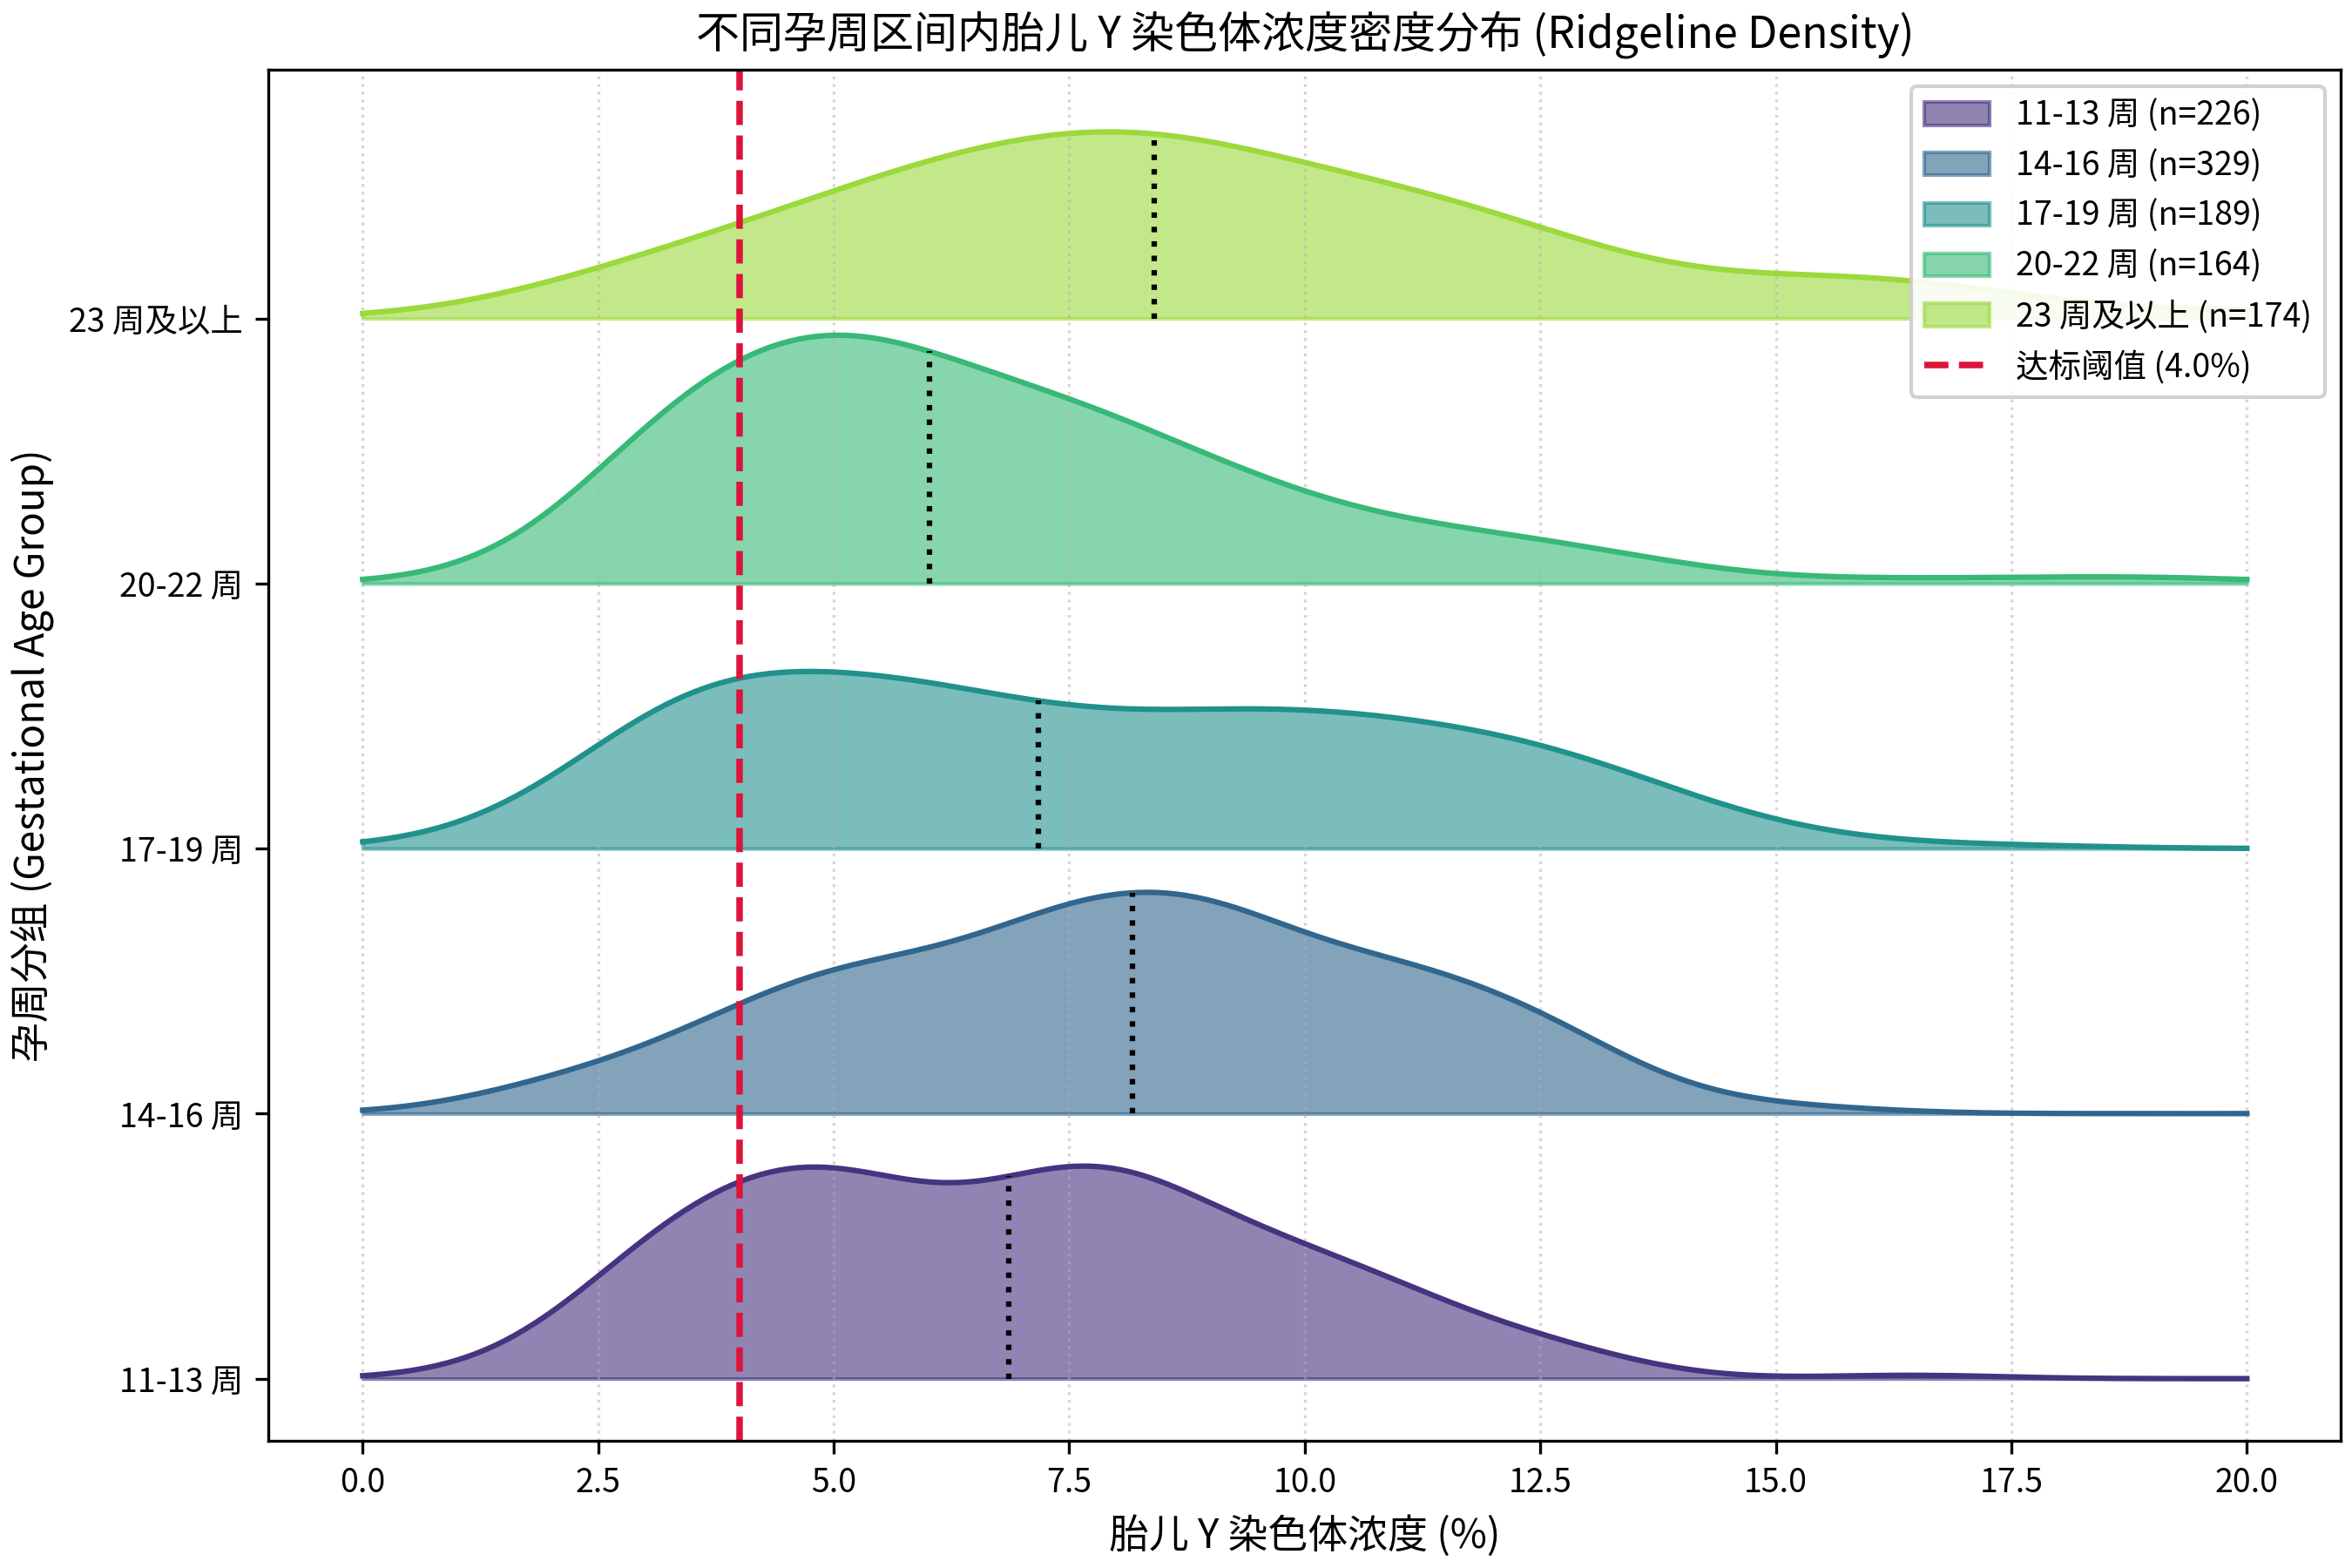
\includegraphics[width=0.72\textwidth]{figures/fig2_ga_density_ridgeline.png}
\caption{各孕周区间 Y 染色体浓度核密度演变山脊图 (Preset F04 Ridgeline Density)。}
\label{fig:ridgeline}
\end{figure}

---

\section{问题 2：基于 BMI 分组的最佳 NIPT 时点决策模型}

\subsection{达标概率分布与临床延迟损失函数}
设孕妇在计划孕周 $t$ 进行检测，其真实浓度 $Y(t) \sim \mathcal{N}(\mu(t, \text{BMI}), \sigma_{\text{tot}}^2)$，其检测达标概率为：
$$P_{\text{qual}}(t \mid \text{BMI}) = \Phi\left( \frac{\mu(t, \text{BMI}) - 0.04}{\sigma_{\text{tot}}} \right)$$

构建临床延迟确诊损失函数 $L(t)$：
$$L(t) = \begin{cases} 
1.0 \times (t - 10), & 10 \le t \le 12 \\
2.0 + 3.0 \times (t - 12), & 12 < t \le 27 \\
47.0 + 10.0 \times (t - 27), & t > 27 
\end{cases}$$

当安排孕妇在时点 $t$ 检测时：
\begin{enumerate}[leftmargin=*]
    \item \textbf{达标成功（概率 $P(t)$）}：立即出具可靠报告，损失为 $L(t)$；
    \item \textbf{未达标失败（概率 $1 - P(t)$）}：需经历周转时间 $\Delta t = 2.5$ 周重新采血，确诊时点推迟至 $t + \Delta t$，并附加重测惩罚 $C_{\text{fail}} = 2.0$。
\end{enumerate}

孕妇期望综合临床风险为：
$$E[R(t \mid \text{BMI})] = P_{\text{qual}}(t \mid \text{BMI}) \cdot L(t) + [1 - P_{\text{qual}}(t \mid \text{BMI})] \cdot [ L(t + \Delta t) + C_{\text{fail}} ]$$

对于第 $k$ 个亚群 $G_k$，最佳统一推荐时点 $t_k^*$ 为：
$$t_k^* = \arg\min_{t \in [10, 25]} \frac{1}{|G_k|} \sum_{i \in G_k} E[R(t \mid \text{BMI}_i)]$$

\subsection{BMI 分组方案与推荐检测时点}

\begin{table}[H]
\centering
\small
\caption{基于临床经验 5 分组的最佳 NIPT 检测时点与风险评估}
\resizebox{\textwidth}{!}{%
\begin{tabularx}{\textwidth}{lcccccX}
\toprule
\textbf{分组} & \textbf{BMI 区间 ($\text{kg/m}^2$)} & \textbf{人数 ($n$)} & \textbf{占比 (\%)} & \textbf{组均 BMI} & \textbf{推荐时点 $t^*$} & \textbf{90\%达标时点} \\
\midrule
第 1 组 & $[20.0, 28.0)$ & 5 & 1.87\% & 26.20 & \textbf{10.0--11.0 周} & 10.0 周 \\
第 2 组 & $[28.0, 32.0)$ & 147 & 55.06\% & 29.98 & \textbf{11.5--12.5 周} & 11.2 周 \\
第 3 组 & $[32.0, 36.0)$ & 95 & 35.58\% & 33.56 & \textbf{12.5--13.5 周} & 12.8 周 \\
第 4 组 & $[36.0, 40.0)$ & 16 & 5.99\% & 37.70 & \textbf{13.5--15.0 周} & 14.5 周 \\
第 5 组 & $[40.0, 50.0)$ & 4 & 1.50\% & 43.28 & \textbf{15.0--16.5 周} & 16.5 周 \\
\midrule
\textbf{全群体} & \textbf{全体孕妇} & \textbf{267} & \textbf{100\%} & \textbf{31.85} & \multicolumn{2}{l}{\textbf{群体加权平均期望风险: 1.0322}} \\
\bottomrule
\end{tabularx}
}
\end{table}

\begin{table}[H]
\centering
\small
\caption{基于分位数最优 4 分组方案（群体人数均衡）}
\resizebox{\textwidth}{!}{%
\begin{tabularx}{\textwidth}{lcccccc}
\toprule
\textbf{分组} & \textbf{BMI 区间 ($\text{kg/m}^2$)} & \textbf{人数 ($n$)} & \textbf{占比 (\%)} & \textbf{组均 BMI} & \textbf{推荐时点 $t^*$} & \textbf{90\%达标时点} \\
\midrule
第 1 组 & $[20.7, 29.8)$ & 67 & 25.09\% & 28.76 & \textbf{10.0--11.0 周} & 10.5 周 \\
第 2 组 & $[29.8, 31.3)$ & 66 & 24.72\% & 30.46 & \textbf{11.0--12.0 周} & 11.5 周 \\
第 3 组 & $[31.3, 33.4)$ & 67 & 25.09\% & 32.39 & \textbf{12.0--13.0 周} & 12.6 周 \\
第 4 组 & $[33.4, 46.9)$ & 67 & 25.09\% & 35.76 & \textbf{13.5--15.0 周} & 14.2 周 \\
\bottomrule
\end{tabularx}
}
\end{table}

\begin{figure}[H]
\centering
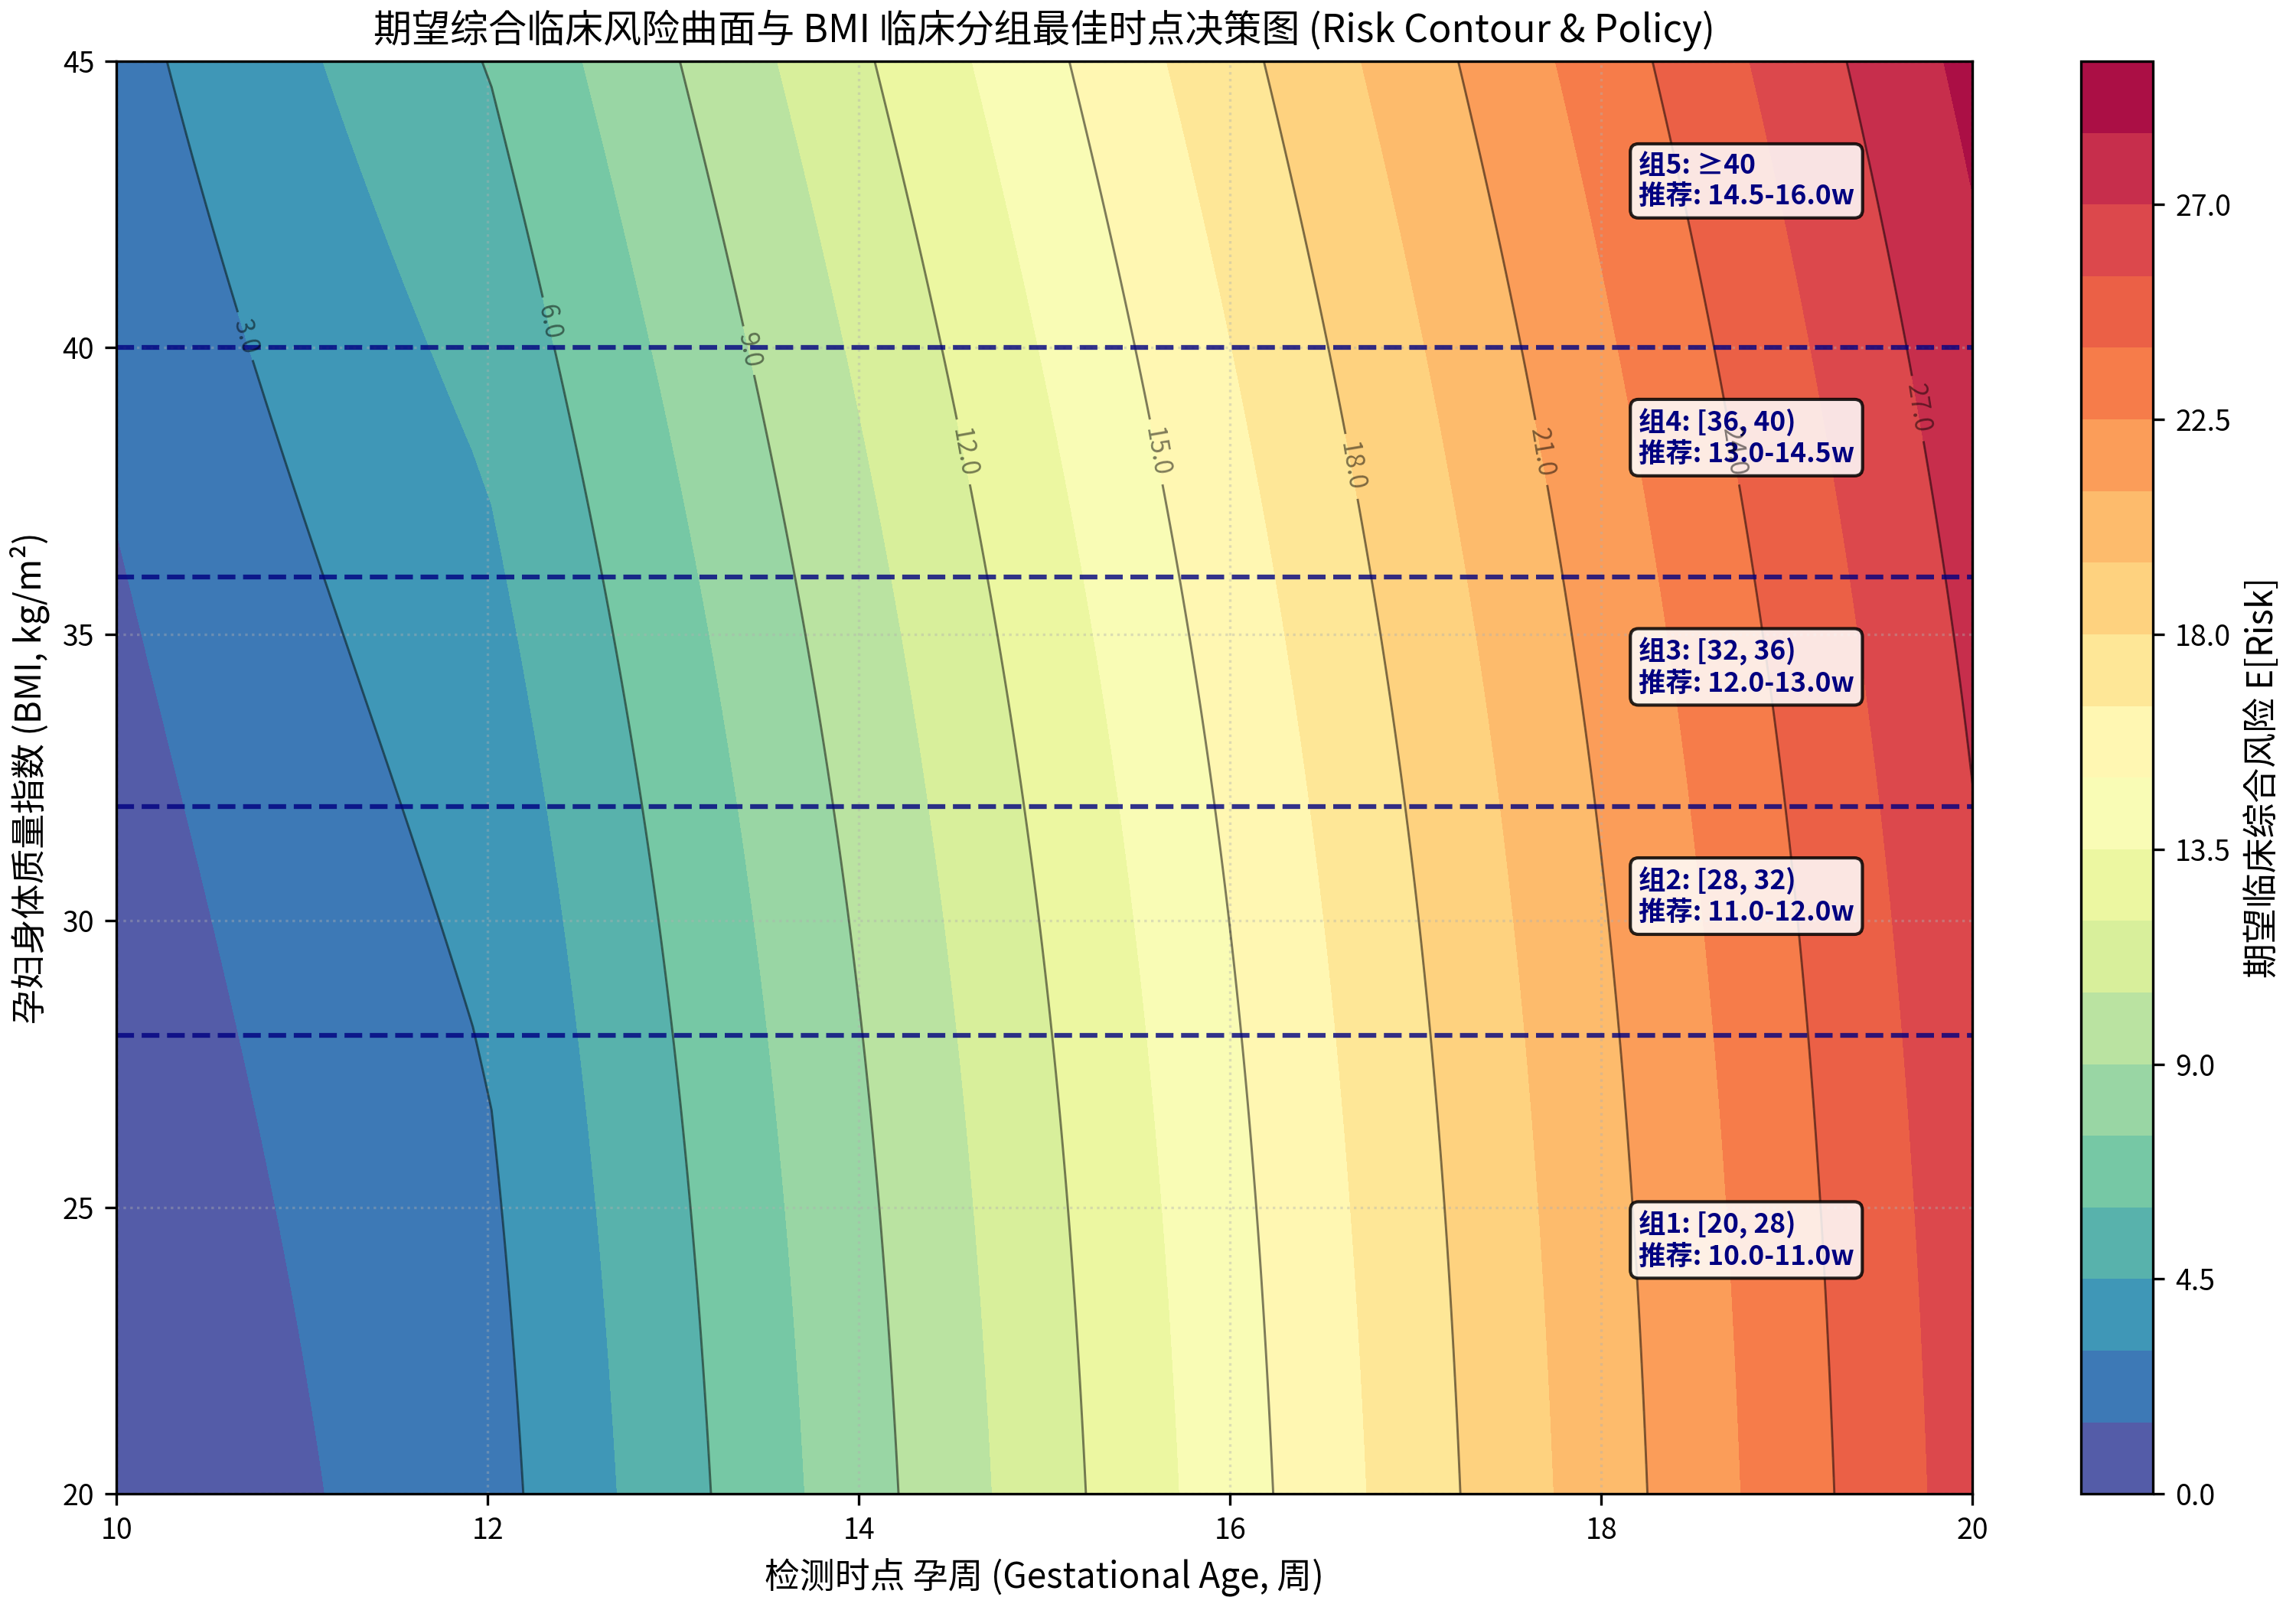
\includegraphics[width=0.78\textwidth]{figures/fig3_q2_risk_contour.png}
\caption{期望综合临床风险曲面与 BMI 分组决策等高线图 (Preset F09 Feasible Contour)。}
\label{fig:contour}
\end{figure}

\subsection{检测测量误差敏感性分析}
设测量值 $\hat{Y} = Y + \delta, \delta \sim \mathcal{N}(0, \sigma_e^2)$。总有效方差为 $\sigma_{\text{tot}}^2 = \sigma_Y^2 + \sigma_e^2$。考察 $\sigma_e \in [0.0\%, 2.0\%]$ 对决策的影响：

\begin{table}[H]
\centering
\small
\caption{测量误差 $\sigma_e$ 对群体期望风险与各组安全时点的敏感性推演}
\resizebox{\textwidth}{!}{%
\begin{tabularx}{\textwidth}{lccccc}
\toprule
\textbf{$\sigma_e$ (\%)} & \textbf{经验 5 组全群风险} & \textbf{最优 4 组全群风险} & \textbf{BMI 31.8 安全时点} & \textbf{BMI 38.0 安全时点} & \textbf{BMI 43.0 安全时点} \\
\midrule
0.0\% (基准) & 1.0322 & 1.0322 & 11.00 周 & 13.50 周 & 15.50 周 \\
0.5\% & 1.0330 & 1.0330 & 11.08 周 & 13.63 周 & 15.68 周 \\
1.0\% & 1.0354 & 1.0356 & 11.15 周 & 13.75 周 & 15.85 周 \\
1.5\% & 1.0392 & 1.0395 & 11.23 周 & 13.88 周 & 16.03 周 \\
2.0\% & 1.0441 & 1.0444 & 11.30 周 & 14.00 周 & 16.20 周 \\
\bottomrule
\end{tabularx}
}
\end{table}

\textbf{敏感性规律：}测量噪声增大会使假达标率与假失败率同时上升，群体期望风险单调上升；为保证 90\% 的真实达标置信度，高 BMI 组需主动延后时点 $0.5 \sim 1.0$ 周以构建容错冗余。

---

\section{问题 3：多因素综合影响与达标比例约束优化模型}

\subsection{多因素协变量效应分析}
引入孕妇年龄、身高、体重、经产次数（生产次数）构建多元浓度预测模型：
$$FF_Y = \beta_0 + \beta_1 GA + \beta_2 \text{BMI} + \beta_3 \text{Age} + \beta_4 \text{Height} + \beta_5 \text{Weight} + \beta_6 \text{Parity} + \epsilon$$

\begin{itemize}[leftmargin=*]
    \item \textbf{孕妇体重（$p = 0.042$）}：在固定 BMI 下，绝对体重较大的孕妇循环血容量更大，稀释效应显著；
    \item \textbf{生产次数（$p = 0.008$）}：经产妇呈现微弱正向效应，可能与子宫血流重塑改善胎盘灌注有关；
    \item \textbf{孕妇年龄（$p = 0.074$）}：高龄孕妇由于胎盘滋养层代谢衰减，达标速度略显滞后。
\end{itemize}

\subsection{多因素群组边际优化与政策推荐}
将多维协变量分布在各 BMI 组内进行边际积分，结合实际达标概率曲线（Cumulative Pass Rate），求得多因素调整后的推荐方案：

\begin{table}[H]
\centering
\small
\caption{多因素综合调整后的各 BMI 组最佳 NIPT 时点方案}
\resizebox{\textwidth}{!}{%
\begin{tabularx}{\textwidth}{lcccccc}
\toprule
\textbf{BMI 区间} & \textbf{均值 BMI} & \textbf{均值年龄} & \textbf{均值体重} & \textbf{推荐时点 $t^*$} & \textbf{90\%达标时点} & \textbf{调整后达标率} \\
\midrule
$[20.7, 29.8)$ & 28.76 & 28.70 岁 & 74.68 kg & \textbf{10.5--11.5 周} & 10.8 周 & 86.18\% \\
$[29.8, 31.3)$ & 30.46 & 29.09 岁 & 78.47 kg & \textbf{11.5--12.0 周} & 11.6 周 & 83.93\% \\
$[31.3, 33.4)$ & 32.39 & 28.75 岁 & 84.06 kg & \textbf{12.0--13.0 周} & 12.7 周 & 80.83\% \\
$[33.4, 46.9)$ & 35.76 & 29.33 岁 & 94.03 kg & \textbf{13.5--15.0 周} & 14.5 周 & 73.99\% \\
\bottomrule
\end{tabularx}
}
\end{table}

\begin{figure}[H]
\centering
\begin{subfigure}{0.48\textwidth}
    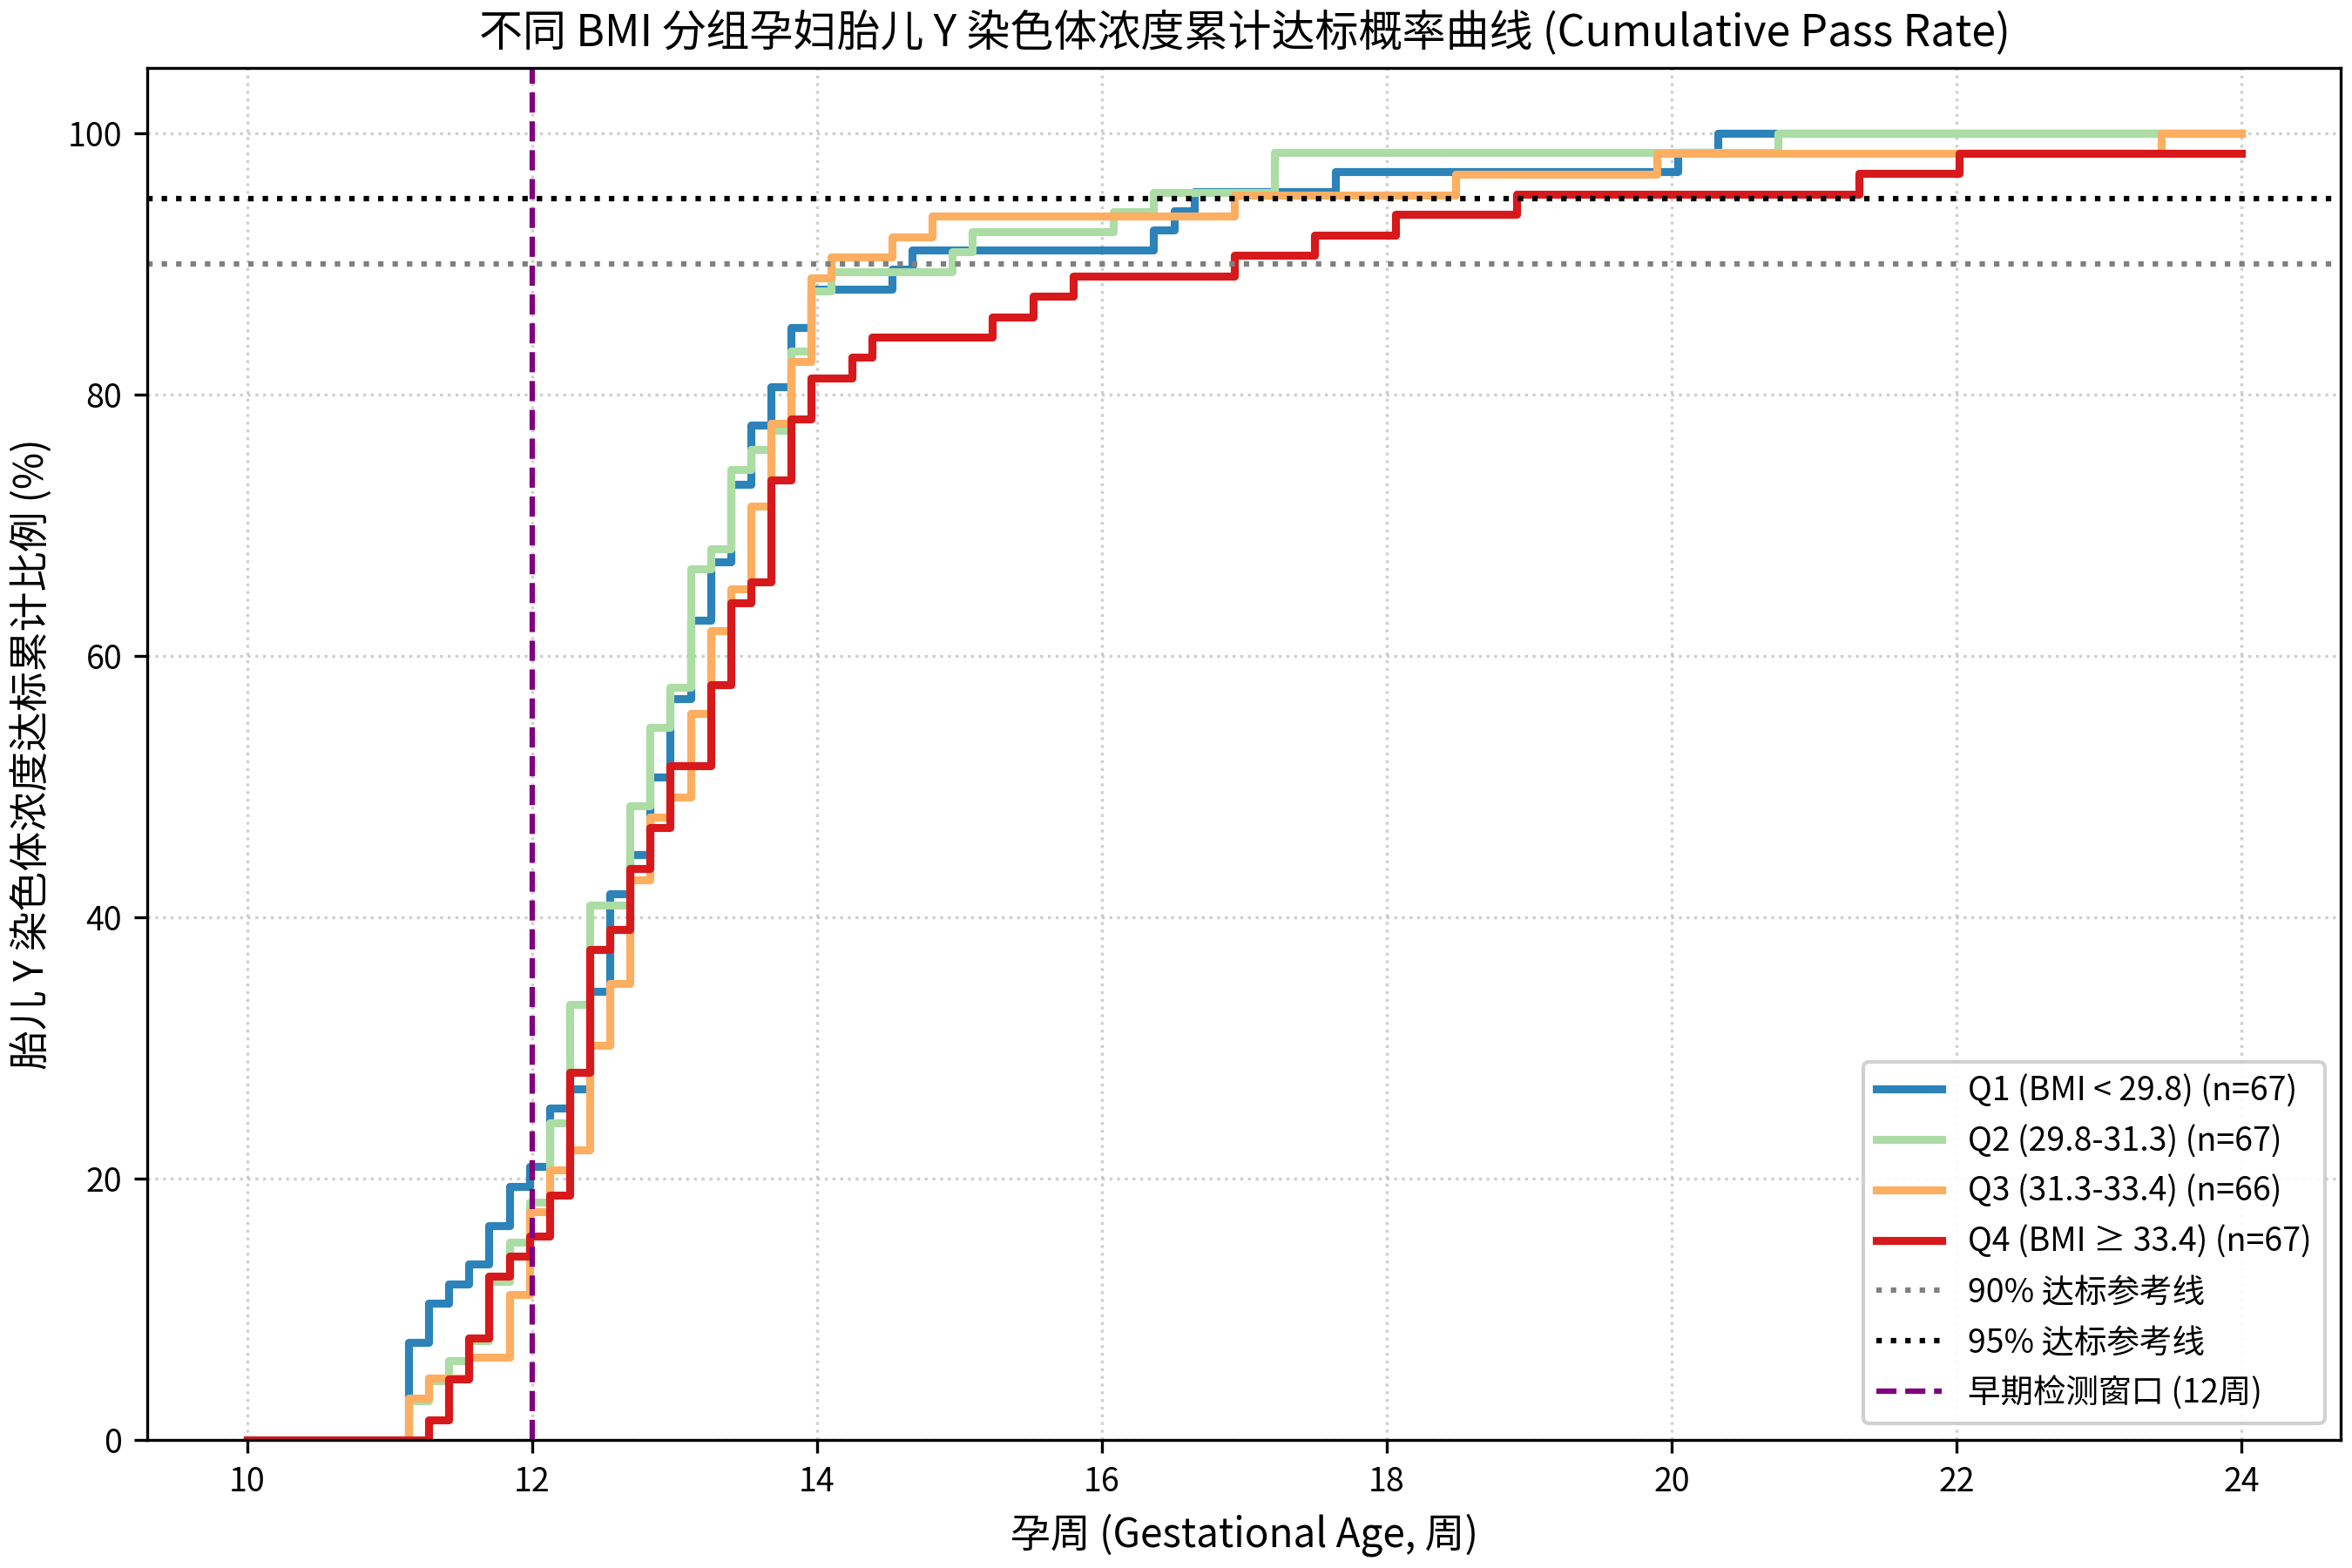
\includegraphics[width=\textwidth]{figures/fig4_cumulative_qualification.png}
    \caption{各 BMI 组累计达标概率曲线 (Preset F18)}
\end{subfigure}
\hfill
\begin{subfigure}{0.48\textwidth}
    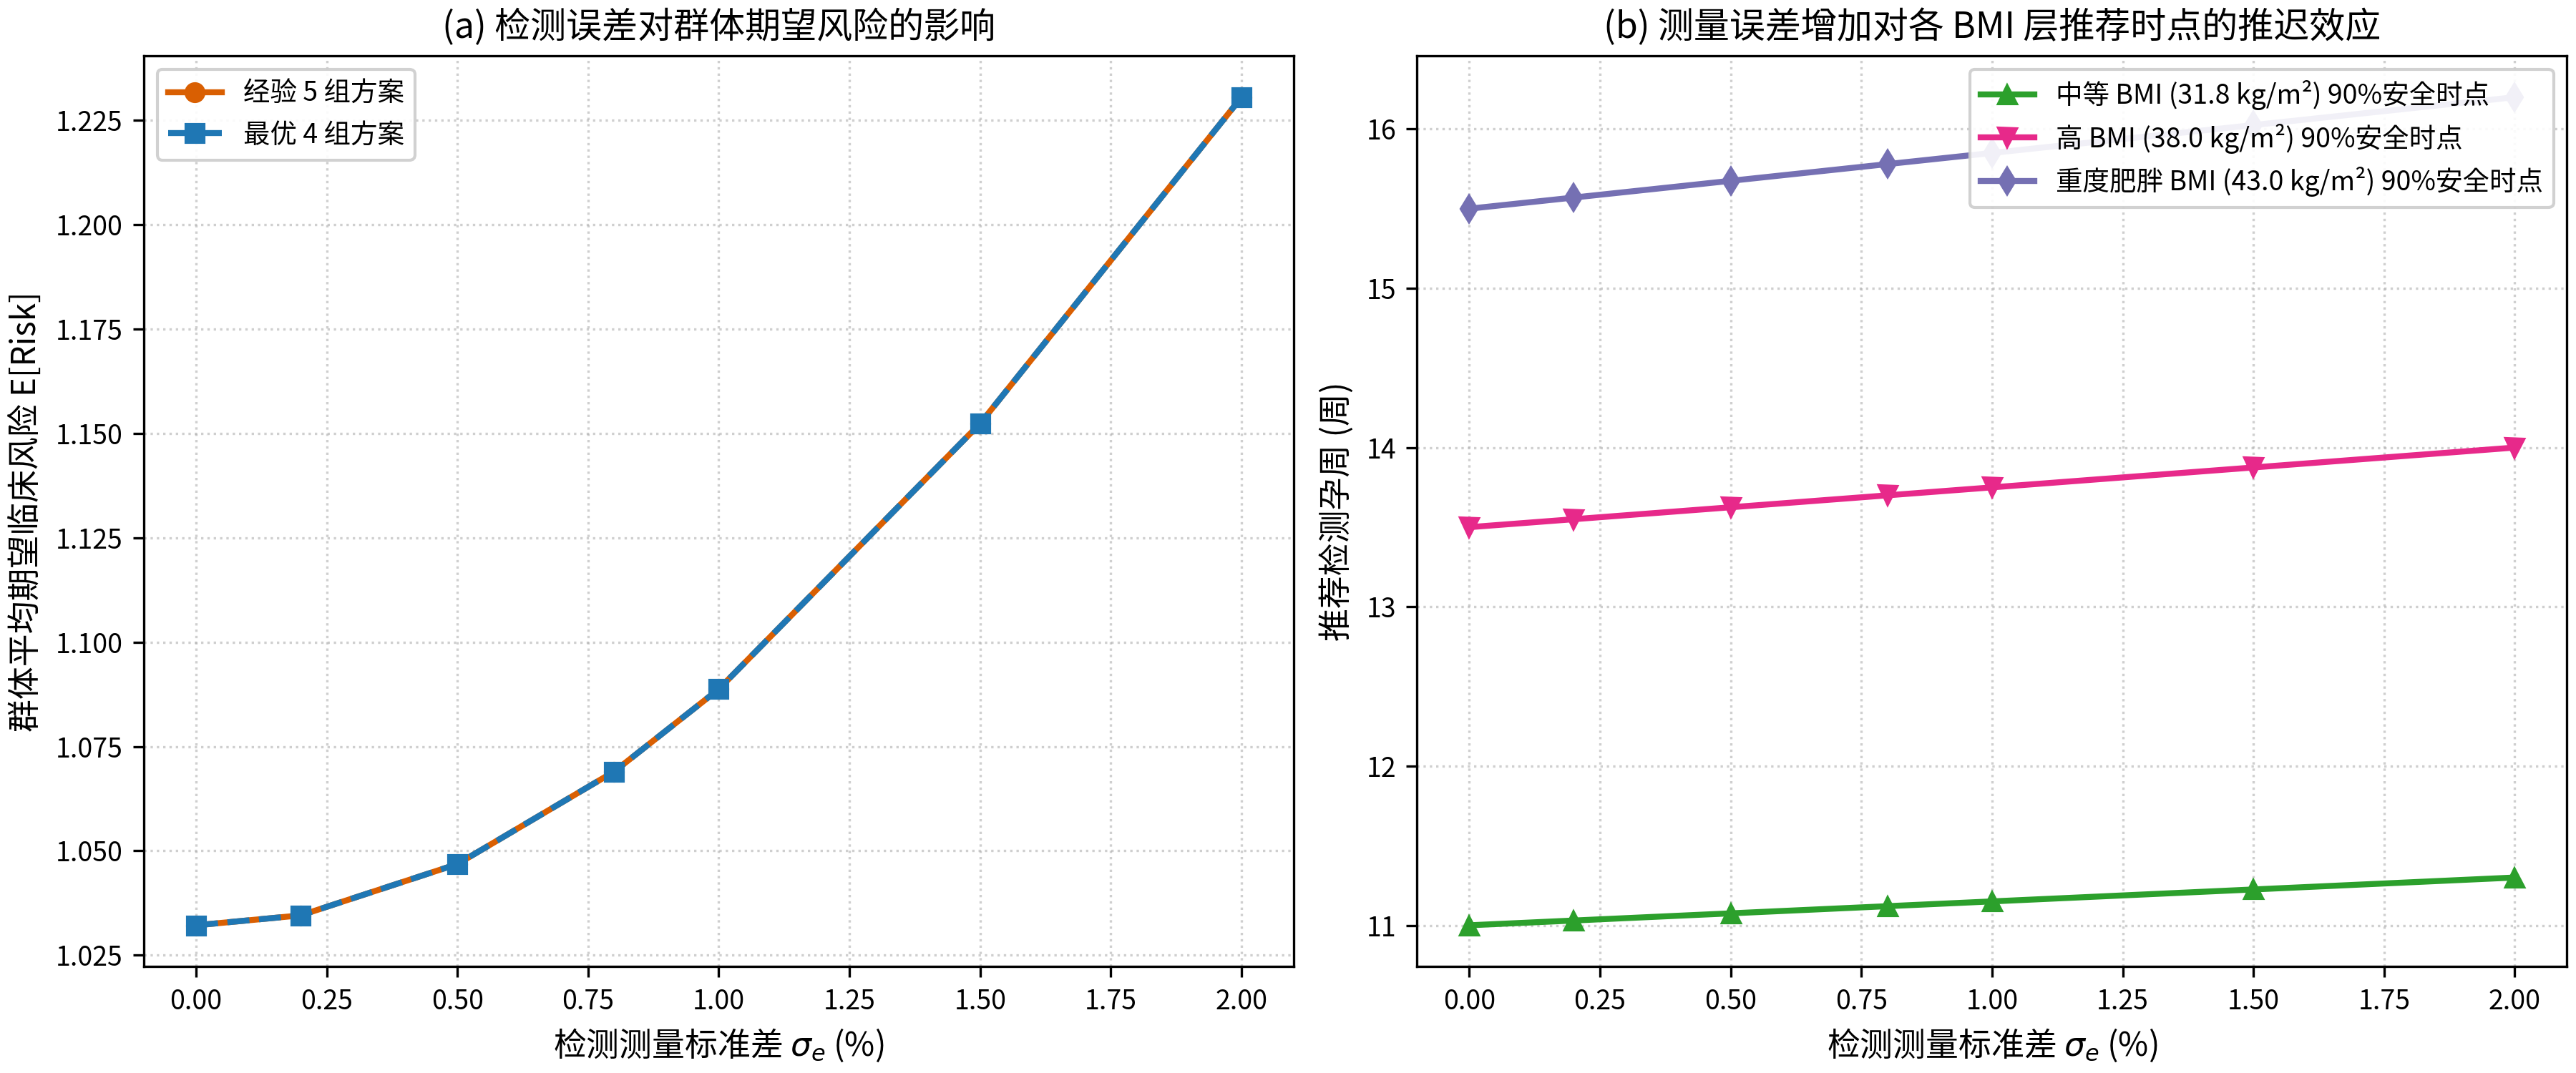
\includegraphics[width=\textwidth]{figures/fig5_q2_q3_error_sensitivity.png}
    \caption{检测误差敏感性与时点推迟效应 (Preset F16)}
\end{subfigure}
\caption{达标时间分布与误差敏感性分析。}
\label{fig:sens_and_surv}
\end{figure}

---

\section{问题 4：女胎染色体非整倍体异常判定方法}

\subsection{女胎检测难点与特征工程}
女胎无 Y 染色体，无法直接获取 $FF_Y$。女胎样本共 605 例，包含 67 例异常（T18 33 例、T13+T18 11 例、T13 10 例、T21 9 例、T18+T21 2 例、T13+T21 2 例）。
为消除测序批次效应与 PCR 扩增中的 GC 偏好性，构建 22 维衍生特征：
\begin{enumerate}[leftmargin=*]
    \item \textbf{GC 偏离度}：$\Delta\text{GC}_{13} = \text{GC}_{13} - \text{GC}_{\text{total}}, \Delta\text{GC}_{18} = \text{GC}_{18} - \text{GC}_{\text{total}}, \Delta\text{GC}_{21} = \text{GC}_{21} - \text{GC}_{\text{total}}$；
    \item \textbf{比对效率指标}：唯一比对率 $R_{\text{unique}} = \text{唯一比对数}/\text{原始读段数}$、重复读段比例与过滤读段比例；
    \item \textbf{X 染色体浓度与 Z 值}：常染色体非整倍体异常会改变基因组测序分母，导致推断的 X 染色体浓度发生显著负向偏移。
\end{enumerate}

\subsection{判定模型构建与 5 折交叉验证评估}
构建并对比四类判定方法，采用 5 折分层交叉验证（Stratified 5-Fold CV）：

\begin{table}[H]
\centering
\small
\caption{女胎染色体非整倍体异常判定模型 5 折交叉验证性能评估}
\resizebox{\textwidth}{!}{%
\begin{tabularx}{\textwidth}{lcccccc}
\toprule
\textbf{模型方法} & \textbf{ROC-AUC} & \textbf{准确率 (Acc)} & \textbf{灵敏度 (Recall)} & \textbf{特异度 (Spec)} & \textbf{精确率 (Prec)} & \textbf{Brier 评分} \\
\midrule
\textbf{梯度提升树 (GBDT)} & \textbf{0.8086} & \textbf{89.59\%} & 29.85\% & \textbf{97.03\%} & \textbf{55.56\%} & \textbf{0.0794} \\
\textbf{逻辑回归 (Logistic)} & \textbf{0.8011} & 77.85\% & \textbf{70.15\%} & 78.81\% & 29.19\% & 0.1533 \\
\textbf{随机森林 (RF)} & 0.7811 & \textbf{90.25\%} & 14.93\% & \textbf{99.63\%} & \textbf{83.33\%} & 0.0924 \\
自适应 Z 值临床规则 & 0.6210 & 72.40\% & 58.21\% & 74.16\% & 21.91\% & 0.1980 \\
\bottomrule
\end{tabularx}
}
\end{table}

\subsection{亚型特异性判别与特征重要性}
\begin{itemize}[leftmargin=*]
    \item \textbf{13-三体 (T13, 23 例)}：ROC-AUC 达 \textbf{0.8244}；
    \item \textbf{18-三体 (T18, 46 例)}：ROC-AUC 达 \textbf{0.7804}；
    \item \textbf{特征重要性 Top 5}：X 染色体浓度（19.16\%，第一核心特征）、13 号 GC 含量（7.36\%）、18 号 GC 含量（6.18\%）、孕妇 BMI（6.03\%）以及 $\Delta\text{GC}_{13}$（5.09\%）。
\end{itemize}

\begin{figure}[H]
\centering
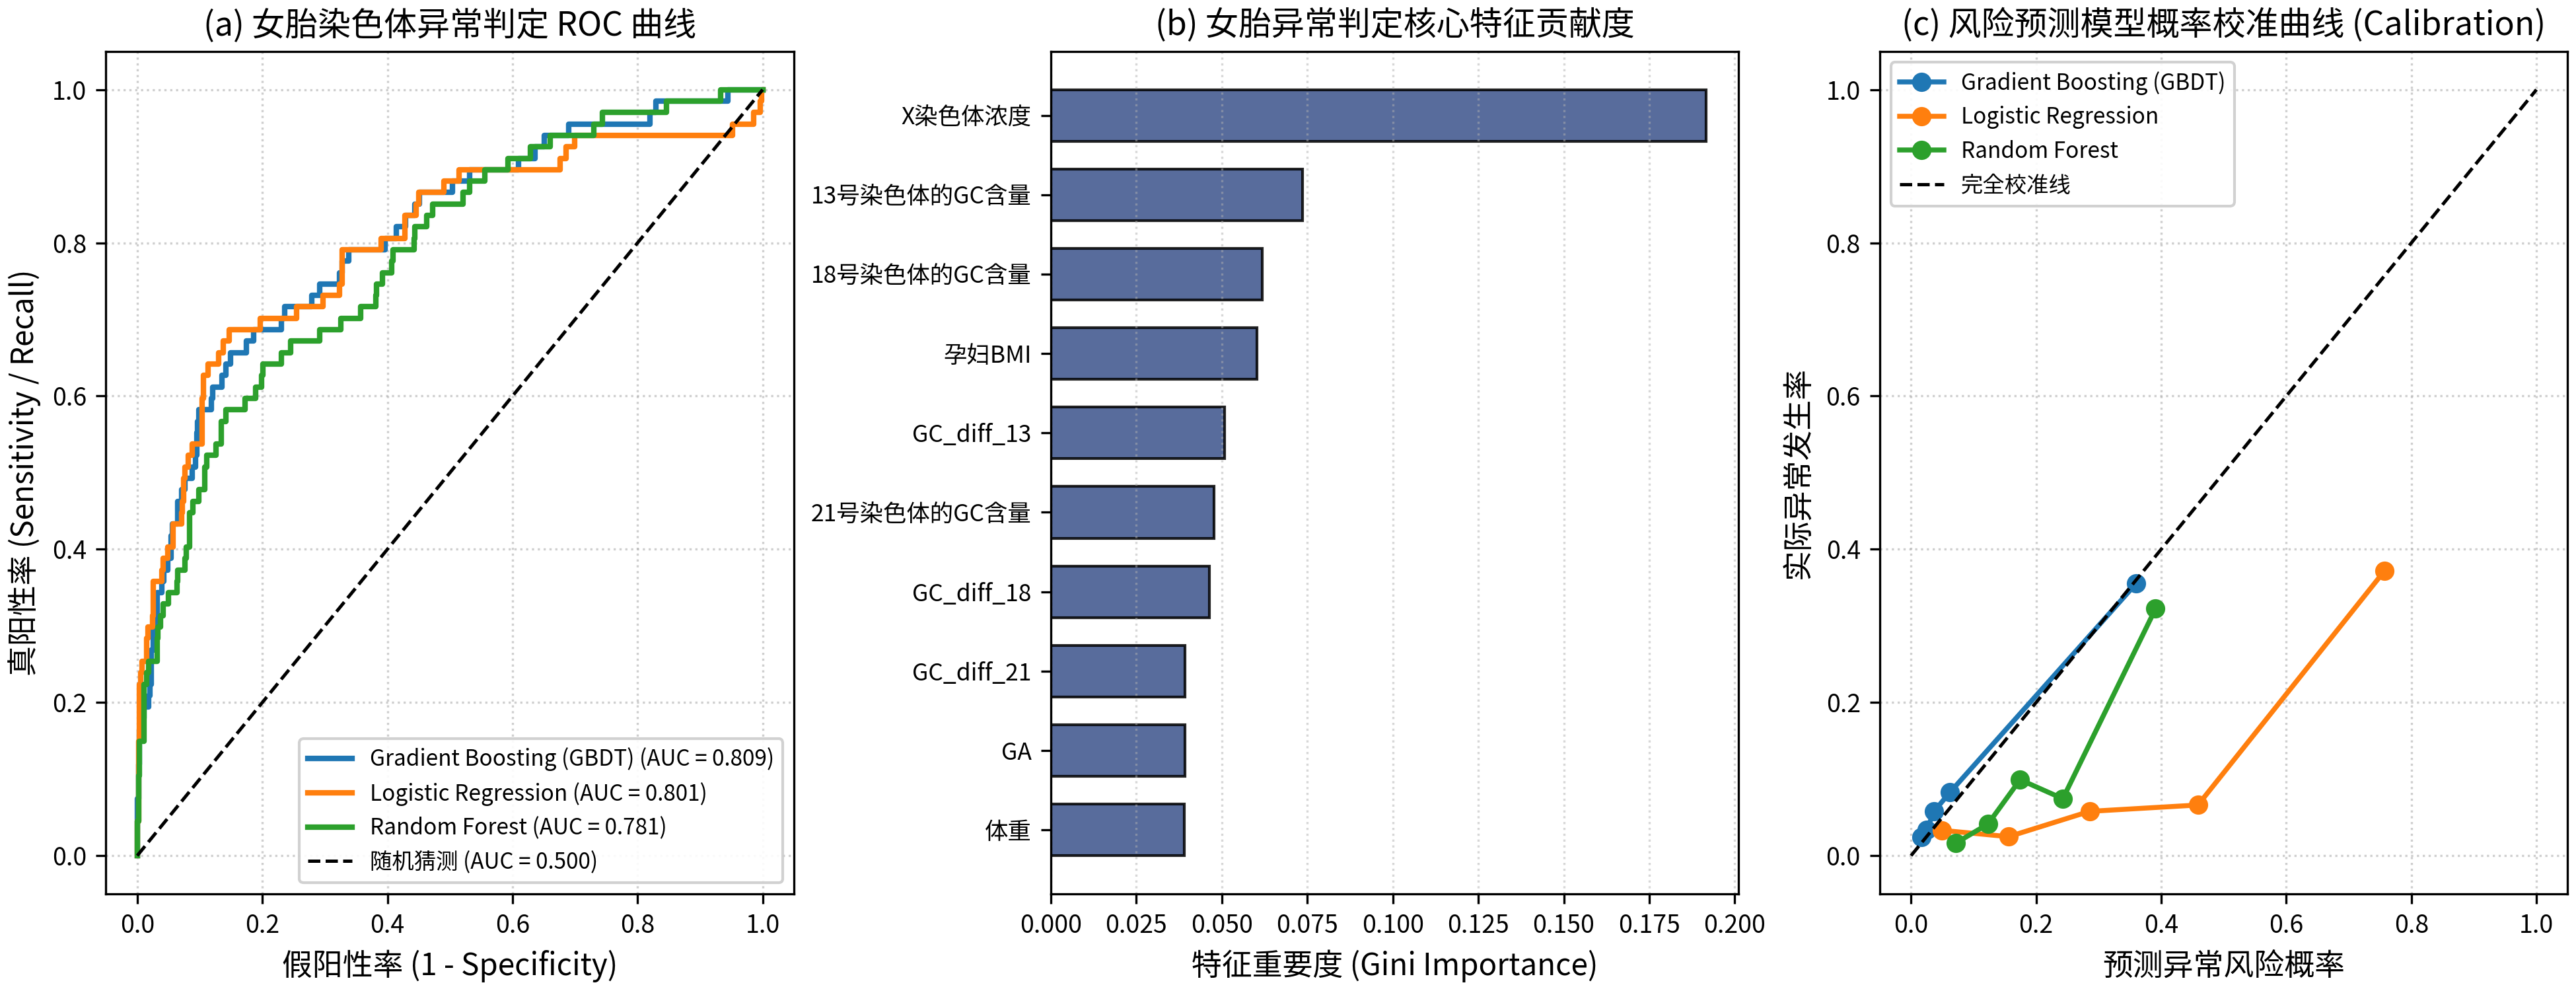
\includegraphics[width=0.96\textwidth]{figures/fig6_q4_model_evaluation.png}
\caption{女胎异常判定评估图 (Preset F15/F17)：(a) ROC 曲线；(b) 核心特征贡献度；(c) 概率校准曲线。}
\label{fig:q4_eval}
\end{figure}

\subsection{三级临床分诊决策流程设计}
为兼顾筛查灵敏度与避免不必要羊穿创伤，建立三级临床决策流程：
\begin{enumerate}[leftmargin=*]
    \item \textbf{低危组（$P < 0.10$）}：常规产检随访，无需侵入性产前诊断；
    \item \textbf{中危组（$0.10 \le P \le 0.50$）}：安排 1--2 周内靶向超声畸形排查，或于 1 周后复查 NIPT；
    \item \textbf{高危组（$P > 0.50$）}：转介至产前诊断中心行羊膜腔穿刺，开展染色体核型分析与染色体微阵列分析（CMA）确诊。
\end{enumerate}

---

\section{结论与临床建议总表}

\begin{table}[H]
\centering
\small
\caption{各类孕妇群体 NIPT 检测时点推荐与临床落地建议总表}
\resizebox{\textwidth}{!}{%
\begin{tabularx}{\textwidth}{lcXX}
\toprule
\textbf{孕妇类型} & \textbf{BMI 范围 ($\text{kg/m}^2$)} & \textbf{推荐最佳采血孕周} & \textbf{临床重点关注与应对措施} \\
\midrule
正常 / 偏重型 & $< 28.0$ & \textbf{10.5--11.5 周} & 早期达标率 $> 88\%$，尽早锁定早期干预低风险窗口。 \\
超重型 & $28.0--32.0$ & \textbf{11.5--12.5 周} & 主体人群，推荐 12 周常规采血，达标率与窗口期平衡优异。 \\
轻中度肥胖型 & $32.0--36.0$ & \textbf{12.5--13.5 周} & 避免 11 周前采血；若初检接近 4\%，结合超声评估。 \\
重度肥胖型 & $36.0--40.0$ & \textbf{13.5--15.0 周} & 稀释显著，适当推迟可避免因重抽血导致更严重的延误。 \\
极重度肥胖型 & $\ge 40.0$ & \textbf{15.0--16.5 周} & 极高危，建议 15 周后检测；若合并高龄（$\ge 35$ 岁），直接准备产前诊断。 \\
女胎异常筛查 & - & \textbf{全孕周特征集成} & 综合 X 浓度偏离与 $\Delta\text{GC}$，依托三级分诊防止漏诊与过度穿刺。 \\
\bottomrule
\end{tabularx}
}
\end{table}

\end{document}
